% Document preamble
\documentclass{article}
\usepackage{lipsum}
\usepackage{graphicx}
\usepackage[table]{xcolor}
\usepackage{xcolor}
\usepackage{colortbl}
\usepackage{titlesec}
\usepackage{soul}
\usepackage{listings}
\usepackage{comment}
% Global settings for listings
    \lstset{
    basicstyle=\ttfamily\small,     % Font size and style for code
    frame=single,                   % Frame around code
    breaklines=true,                % Enable line breaks
    captionpos=b,                   % Position of caption
    numbers=left,                   % Line numbers on the left
    numberstyle=\tiny\color{gray},  % Style for line numbers
    stepnumber=1,                   % Step for line numbers
    numbersep=5pt,                  % Distance between line numbers and code
    showstringspaces=false,         % Do not show spaces in strings
    commentstyle=\color{green},     % Comment style
    keywordstyle=\color{blue},      % Keyword style
    stringstyle=\color{red},        % String style
}
\usepackage{amsmath}
\usepackage{circuitikz}
\usepackage{tikz}
\usetikzlibrary{positioning, shapes.geometric, arrows}
\usepackage{float}
\usepackage{caption}
\usepackage{url}
\usepackage{pgfplots,pgfplotstable}
\pgfplotsset{compat=1.18}
\date{\today}

%Packages for costum tables
\usepackage{booktabs, multirow}
\usepackage{changepage,threeparttable}

% Set the document layout
\usepackage{multicol}
\usepackage{geometry}
\geometry{margin=1.5cm}

% Set the authors and affiliation
\usepackage{authblk}
\author{Kasandikromo Guillian}
\author{Karg Timothy}
\author{Uraicia Sewpersad}
\affil{Vanguard Community College - Department of Engineering}

% Modify the authors and affilition text
\renewcommand\Authfont{\bfseries\fontsize{9}{14}\selectfont}
\renewcommand\Affilfont{\fontsize{12}{14}\selectfont}

% Set the header of the document
\usepackage{fancyhdr}
\pagestyle{fancy}
\fancyhf{}
\fancyhead[L]{\fontsize{8}{12}\selectfont Vanguard Community College}
\fancyhead[C]{\fontsize{8}{12}\selectfont \date{\today}}
\fancyhead[R]{\fontsize{8}{12}\selectfont Page \thepage}

% Modify the header lenght, width and position
\newlength\FHleft
\newlength\FHright
\setlength\FHleft{1cm}
\setlength\FHright{0cm}
\setlength{\headheight}{25pt}

% Set the separation lenght of the columns
\setlength{\columnsep}{1cm}

% Set the titel of the document
\title{\huge \bfseries
    Monitoring Energy Consumption using Arduino}

% Redefine the section numbering format
\renewcommand{\thesection}{\Roman{section}.}
\renewcommand{\thesubsection}{\roman{subsection}.}
\titlespacing*{\section}{0pt}{1cm}{0.5cm}
\titlespacing*{\subsection}{0pt}{0.5cm}{2pt}
\titleformat{\section}
  {\bfseries\large\centering}{\thesection}{1em}{}
\titleformat{\subsection}
  {\normalsize\centering\itshape}{\thesubsection}{1em}{}

\begin{document}
    \begin{multicols}{2}
        \maketitle
        \thispagestyle{fancy}
       \begin{abstract}
        \setlength{\baselineskip}{1.2\baselineskip}
        \noindent
        \makebox[\linewidth]{
            \begin{minipage}{0.48\textwidth}
            This project explains how to set up an Arduino-based system to measure and monitor energy use, making the data accessible in real-time through cloud storage and a web app. As energy optimization becomes more important, this setup provides accurate and easily accessible energy data to help users make informed decisions.

The system uses an Arduino microcontroller with a YHDC Current Transformer SCT-013-000 sensor to measure current. The Arduino converts this data into energy consumption readings in kilowatt-hours (kWh) after first calculating power (watts) and then energy (watt-seconds). Every 10 seconds, this data is sent to a cloud-based PostgreSQL database via a Python script, which connects to the Arduino’s serial output.

To make the data easy to view and analyze, a web app built with Flask and Dash lets users filter data by month or day to explore detailed energy usage patterns. The app also updates automatically, so the latest measurements are always available. With data stored in the cloud, users can monitor energy use from anywhere, helping them identify opportunities to save energy.

Overall, this system combines Arduino's compatibility with various sensors and the cloud’s accessibility, creating a reliable and scalable solution for tracking energy usage in real time.

            \end{minipage}}
        \end{abstract}

        % Set sections and bibliography
        \section{Introduction}

This project aims to develop and deploy an Energy Monitor system, designed to provide real-time energy consumption data for a residential setting. The core component of the system is an Arduino-based microcontroller, responsible for collecting and processing energy consumption data from various sensors. This data is then transmitted to a web server, allowing for remote monitoring and analysis. 

The web application, built using Python and Flask, provides a user-friendly interface to visualize energy consumption patterns, identify potential areas for energy savings, and generate insightful reports. This project leverages the power of open-source technologies to create a cost-effective and customizable solution for energy monitoring.

Key Features:
\begin{itemize}
    \item Real-time monitoring: The system provides up-to-date energy consumption data.
    \item Remote access: Users can access and analyze data from anywhere with an internet connection.
    \item Data visualization: The web application offers various visualization tools for easy data interpretation.
    \item Energy efficiency insights: The system helps identify areas for energy savings and optimization.
\end{itemize}

This document will detail the system's architecture, hardware implementation, software development, and deployment process. It will also include a comprehensive evaluation of the system's performance and potential future enhancements.
        \section{Materials}
\lipsum[1-1]
\subsection{Arduino Micro-controller}

\begin{itemize}
    \item Microcontroller: The heart of the project. It processes the data received from sensors, performs calculations, and controls other components.
    \item Digital and Analog Pins: These pins are used to connect sensors and actuators. Digital pins provide high or low signals, while analog pins can read varying voltage levels.
    \item Power Supply: The board can be powered by a USB cable or an external power supply.
    \item Serial Communication: The board can communicate with a computer or other devices using a serial connection.
\end{itemize} 

\subsection{YHDC Current Transformer SCT-013-000}
    \begin{minipage}{\linewidth}
\begin{figure}[H]
\centering
    \begin{circuitikz}
        \tikzstyle{every node}=[font=\small]
        \draw [](1.25,11.5) to[short] (3,11.5);
        \draw [](1.25,11.5) to[short, -o] (0.75,11.5);
        \draw [->, >=Stealth] (1.75,11.5) -- (2,11.5);
        
        \draw [](3,11.5) to[short] (3,10.75);
        \draw [](3,11) to[short] (3,10.5);
        \draw (3,10.5) to[L ] (5,10.5);
        
        \draw [](5,10.5) to[short] (5,11.5);
        \draw [](5,11.5) to[short] (6.5,11.5);
        \draw [](6.5,11.5) to[short, -o] (7,11.5) ;
        \draw [->, >=Stealth] (6,11.5) -- (6.25,11.5);
        \draw (2.75,9.5) to[L ] (5.25,9.5);
        
        \draw[] (5.25,9.5) to[short] (5,9.5);
        
        \draw[] (5,9.5) to[short] (4.75,9.5);
        \draw [, dashed] (2.75,11) rectangle  (5.25,9.25);
        \draw [](2.75,9.25) to[short] (2.75,8.75);
        \draw [](2.75,8.75) to[short] (2.75,8.25);
        
        \draw [](5.25,9.25) to[short] (5.25,8.25);
        \draw[] (5.25,8.25) to[short] (4.5,8.25);
        \node at (4.5,8.25) [circ] {};
        \draw [](4.5,8.25) to[short] (4.5,6.25);
        \node at (2.75,8.25) [circ] {};
        
        \draw [](2.75,8.25) to[short] (2.75,5.75);
        \draw (2.25,7.25) to[C] (1.5,7.25);
        \node at (2.75,7.25) [circ] {};
        \draw (2.25,7.25) to[C] (1,7.25);
        \draw [](2.75,5.75) to[short] (2.75,5.5);
        \draw [](2.75,5.5) to[short] (2.75,5.25);
        \node at (2.75,5.25) [circ] {};
        \draw (2.75,5.25) to[R] (4.75,5.25);
        \draw (2.25,5.25) to[R] (1,5.25);
        \draw [](2.25,5.25) to[short] (2.75,5.25);
        \draw [](2.25,7.25) to[short] (2.75,7.25);
        \draw[] (1,5.25) to[short] (0.75,5.25);
        \draw[] (1,7.25) to[short] (0.75,7.25);
        \draw[] (0.75,5.25) to[short] (0.5,5.25);
        \draw[] (0.75,7.25) to[short] (0.5,7.25);
        \node at (0.5,7.25) [circ] {};
        \node at (0.5,5.25) [circ] {};
        \draw [](0.5,5.25) to[short] (0.5,7.25);
        \draw [](0.5,7.25) to[short] (0.5,8.25);
        \draw [](0.5,5.25) to[short] (0.5,4);
        \draw [](2.75,5.25) to[short] (2.75,4.25);
        \draw [](2.75,4.25) to[short] (2.75,4);
        \draw [](4.5,6.25) to[short] (4.5,4);
        \draw [](4.5,5.25) to[short] (5,5.25);
        \draw [](4.75,5.25) to[short] (5.5,5.25);
        \draw [](5.5,5.25) to[short] (5.5,4);
        \node [font=\small] at (1.75,11.75) {Heavy line current};
        \node [font=\small] at (6.75,10) {Current transformer};
        \node [font=\small] at (4,9) {Secondary};
        \node [font=\small] at (4,11.25) {Primary};
        \node [font=\small] at (6,11.75) {To load};
        \node [font=\small] at (1.75,8) {C1 10$\mu$F};
        \node [font=\small] at (1.75,5.75) {R1 10k$\Omega$};
        \node [font=\small] at (3.75,5.75) {R2 10k$\Omega$};
        \draw [](2.75,8.25) to[short] (4.5,8.25);
        \node [font=\small] at (6.25,8.75) {C.T Output};
        \node [font=\small, rotate around={270:(0,0)}] at (0.25,4.5) {Arduino GND};
        \node [font=\small, rotate around={270:(0,0)}] at (4.25,4) {Arduino input};
        \node [font=\small, rotate around={270:(0,0)}] at (5.75,4.5) {Arduino 5V DC};
        \node [font=\small, rotate around={270:(0,0)}] at (2.5,4.5) {Mid-point};
        \draw [](5.5,3.75) to[short, o-] (5.5,4) ;
        \draw [](0.5,3.75) to[short, o-] (0.5,4) ;
        \draw [](4.5,3.75) to[short, o-] (4.5,4) ;
        \draw [](2.75,4) to[short] (2.75,3.75);
    \end{circuitikz}
    \caption{Current transformer circuit with Arduino}
    \label{fig:CT - Sensor}
\end{figure}
\vspace{2pt}
\end{minipage}
\begin{itemize}
    \item  Non-invasive Measurement: It measures the current flowing through a wire without physically breaking the circuit.
    \item Magnetic Induction: It works based on the principle of electromagnetic induction.
    \item Output Signal: It produces a small AC voltage proportional to the current flowing through the wire.
    \item Safety: It allows for safe measurement of high currents without the risk of electric shock.
\end{itemize}

\subsection{Liquid Crystal Display}
\begin{itemize}
    \item Display: It displays information like voltage, current, power consumption, and other relevant data.
    \item Backlight: It provides illumination for better visibility.
    \item Interface: It connects to the Arduino board through digital pins to receive and display data. 
    \item Types: There are various types of LCDs, including character LCDs and graphic LCDs. \cite{OpenEnergyMonitor}
\end{itemize} 

\subsection{ Other Potential Components:}
\begin{itemize}
    \item Voltage Sensor: Measures the voltage entering the circuit.
    \item Temperature Sensor: Monitors the temperature of the system or environment.
    \item Power Supply: Provides the necessary power for the Arduino and other components.
    \item Resistors: Used to limit current and divide voltage.
    \item Capacitors: Used to filter noise and store energy.
\end{itemize}
        \section{System Design}
\label{sec:system_design}

\noindent The energy monitoring system consists of three main components:
the Arduino microcontroller, the YHDC Current Transformer (CT) SCT-013-000 sensor, and a cloud-based PostgreSQL database accessible through a web application. Each component plays a vital role in capturing, processing, storing, and displaying energy consumption data in real-time.

\subsection{Hardware Components}
\noindent The system's hardware includes:
\begin{itemize}
    \item \textbf{Arduino Microcontroller:} The Arduino serves as the primary data collection unit, converting analog signals from sensors to digital data for processing. It calculates the instantaneous power and energy usage based on current measurements from the CT sensor.
    \item \textbf{YHDC SCT-013-000 Current Transformer Sensor:} This non-invasive sensor measures the AC current flowing through a wire. It generates an analog signal proportional to the current, which is read by the Arduino's analog input.
    \item \textbf{AC-to-AC Power Adapter:} To measure AC voltage, an AC-to-AC adapter is used. This adapter steps down the AC voltage to a safe level compatible with the Arduino's analog input, allowing it to monitor real-world voltage values accurately.
\end{itemize}

\subsection{Software Components}
\noindent The software components of the system include:
\begin{itemize}
    \item \textbf{Data Processing on Arduino:} The Arduino processes signals from the CT sensor and calculates power by combining current and voltage values. The calculated energy data is sent to a local SQLite database, which is later synced with a cloud database.
    \item \textbf{Python Data Transfer Script:} A Python script interfaces with the Arduino's serial monitor and transfers the processed data to a cloud-based PostgreSQL database at intervals of 10 seconds.
    \item \textbf{Flask Web Application:} A Flask-based application with Dash visualizes the data, allowing users to filter by month and day to observe consumption trends. This user interface provides an accessible and flexible way to monitor energy usage over time.
\end{itemize}

\subsection{Data Flow and Operation}
\begin{minipage}{\linewidth}
    \centering
    \begin{tikzpicture}[
        % Define styles for the components
        block/.style={rectangle, draw, text centered, rounded corners, minimum height=2em, minimum width=3cm, fill=gray!10},
        arrow/.style={thick,->,>=stealth},
        sensor/.style={diamond, draw, text centered, minimum height=2em, minimum width=2em, fill=blue!10},
        storage/.style={cylinder, draw, shape border rotate=90, aspect=0.25, minimum height=2cm, minimum width=1cm, fill=green!20}
    ]
    
    % Define nodes
    \node[block] (power) {Power Source};
    \node[sensor, below=of power] (sensor) {CT Sensor};
    \node[block, below=of sensor] (arduino) {Arduino Microcontroller};
    \node[storage, below=of arduino] (database) {Cloud Database};

    % Draw arrows
    \draw[arrow] (power) -- (sensor) node[midway, right] {AC Current};
    \draw[arrow] (sensor) -- (arduino) node[midway, right] {Analog Signal};
    \draw[arrow] (arduino) -- (database) node[midway, right] {Energy Data (kWh)};

    % Add annotations
    \node[below=0.3cm of database, align=center] {Data stored in PostgreSQL database \\ accessible by web app};
    \end{tikzpicture}
    \captionof{figure}{\small \indent Process Flow Diagram of the Energy Monitoring System}
    \vspace{0.5cm}
    \label{fig:PFD}
\end{minipage}
\noindent The system operates as follows:
\begin{enumerate}
    \item The Arduino reads analog signals from the CT sensor and the AC-to-AC adapter.
    \item It processes these signals, calculates energy consumption in watt-seconds (later converted to kWh), and sends the data to the Python script.
    \item The Python script logs the data in a local SQLite database, which then syncs to a PostgreSQL cloud database every 10 seconds.
    \item The web app fetches the latest data from the cloud database, displaying it with interactive filters for user analysis.
\end{enumerate}

\noindent This modular design, combining hardware and software elements, enables real-time, remote monitoring of energy usage.

        \section{Measuring AC Voltage with an AC to AC power adapter}
\lipsum[1-2]
\begin{minipage}{\linewidth}
\begin{table}[H]
    \centering
    \caption{AC-AC Voltage Transformator Data }
    \label{tab:voltage transformator }
    \small
    \begin{tabular*}{\linewidth}{@{\extracolsep{\fill}}ccc}
    \textbf{V (input) (V)} &\textbf{I (mA)} &\textbf{V(output) (mV)} \\\midrule
    10 &0.59 &3.6 \\
    20 &1.15 &8.6 \\
    30 &1.7 &12.8 \\
    40 &2.25 &16.9 \\
    50 &2.8 &21.2 \\
    60 &3.4 &25.3 \\
    70 &3.96 &29.6 \\
    80 &4.52 &33.6 \\
    90 &5 &38 \\
    100 &5.67 &42.2 \\
    110 &6.21 &46.4 \\
    120 &6.77 &51 \\
    130 &7.38 &55.2 \\
    140 &7.9 &59.1 \\
    \bottomrule
    \end{tabular*}
\end{table}
\begin{tikzpicture}
    \begin{axis}[
    title={AC-AC Voltage Transformator Input vs. Output},
    ticklabel style={font=\scriptsize},
    xlabel={V (input) (V)},
    ylabel={V(output) (mV)},
    xmin=0, xmax=150,
    ymin=0, ymax=60,
    xtick={0,10,20,30,40,50,60,70,80,90,100,110,120,130,140},
    ytick={0,10,20,30,40,50,60},
    legend pos=north west,
    ymajorgrids=true,
    grid style=dashed,
    xmajorgrids=false
]
    \addplot[
        color=red!80,
        mark=circle,
    ]
    coordinates {
        (10,3.6)(20,8.6)(30,12.8)(40,16.9)(50,21.2)(60,25.3)(70,29.6)(80,33.6)(90,38)(100,42.2)(110,46.4)(120,51)(130,55.2)(140,59.1)
    };
    \addlegendentry{V(output) (mV)}
    \label{fig:V in-out}
    \end{axis}
\end{tikzpicture}
\end{minipage}
        \bibliographystyle{IEEEtran}
        \bibliography{Reference}

        \end{multicols}



        % Code listings
        %\section{Code Listings}

The application consists of the following components:
\begin{itemize}
    \item \textbf{Backend (app.py):} Built with Flask, it fetches data from a PostgreSQL database, processes it, and serves it to the front-end.
    \item \textbf{Frontend (index.html):} A responsive HTML page styled with CSS, allowing users to select filters and view energy data in a Plotly graph.
    \item \textbf{CSS (style.css):} Defines styles for the HTML elements to make the dashboard user-friendly and visually appealing.
\end{itemize}
% Define custom colors
\definecolor{ArduinoBlue}{rgb}{0.0, 0.0, 1.0}
\definecolor{ArduinoGreen}{rgb}{0.0, 0.5, 0.0}
\definecolor{ArduinoRed}{rgb}{0.85, 0.0, 0.0}
\definecolor{ArduinoGray}{rgb}{0.5, 0.5, 0.5} 

% Define Arduino style
\lstdefinestyle{Arduino}{
  language=C++,
  backgroundcolor=\color{white},                % White background
  basicstyle=\ttfamily\small,                   % Use monospace font (default Arduino IDE font)
  keywordstyle=\color{ArduinoBlue}\bfseries,    % Blue color for keywords (e.g., void, int)
  commentstyle=\color{ArduinoGreen}\itshape,    % Green color for comments (e.g., // comment)
  stringstyle=\color{ArduinoRed} \itshape,      % Dark red color for strings
  numberstyle=\tiny\color{ArduinoGray},         % Small gray line numbers
  numbersep=5pt,                                % Distance between numbers and code
  frame=single,                                 % Border around code
  breaklines=true,                              % Wrap long lines
  showstringspaces=false,                       % Do not show spaces in strings
  captionpos=b,                                 % Place caption at the bottom
  numbers=left,                                 % Show line numbers
  stepnumber=1,                                 % Step through line numbers
  morekeywords={void, int, float, double, long, char, bool, for, while, if, else}, % Common Arduino keywords
  escapeinside={\%*}{*)},                       % Allow LaTeX commands inside listings
  literate={-}{-}{1},                            % Fix the minus signs in code
  identifierstyle=\color{ArduinoGray},          % Color for identifiers (variables, functions)
}

\subsection{Arduino Code Breakdown}

\subsubsection{Initializing Libraries and Variables}
\begin{lstlisting}[style=Arduino]
#include "EmonLib.h"
EnergyMonitor emon1;  // Create an instance

// Variables for measurements
double ACV;
double Irms;
double Power;
double Energy = 0.0;
double totalEnergy = 0.0;
double kWh = 0.0;
\end{lstlisting}

\subsubsection{Setup Function}
\begin{lstlisting}[style=Arduino]
void setup() {
  Serial.begin(9600);  
  emon1.current(A0, 20.85);  
  emon1.voltage(A2, 171.36, 1.7);  
}
\end{lstlisting}

\subsubsection{Main Loop for Measurements}
\begin{lstlisting}[style=Arduino]
void loop() {
  double Irms = emon1.calcIrms(1480); 
  double ACV = 127.0;  // Assume constant AC voltage of 127V
  double Power = Irms * ACV; 
  
  // Print the power to the serial monitor
  Serial.print("Power: ");
  Serial.println(Power);
}
\end{lstlisting}

\subsubsection{Energy Calculation and Printing Data}
\begin{lstlisting}[style=Arduino]
  // Calculate energy in watt-seconds for the 10-second interval
  Energy = Power * (MEASURE_INTERVAL / 1000.0);   
  totalEnergy += Energy;                          

  // Calculate kWh from total energy (in watt-seconds)
  kWh = totalEnergy / 3600000.0;  

  // Print data in CSV format for Python parsing
  printData();
\end{lstlisting}

\subsubsection{Simulating Time and Printing Data}
\begin{lstlisting}[style=Arduino]
void printData() {
  // Simulate incrementing time (1 measurement every 10 seconds)
  seconds += 10; 

  // Adjust minutes and hours based on seconds overflow
  if (seconds >= 60) {
    seconds -= 60;
    minutes++;
  }
  if (minutes >= 60) {
    minutes -= 60;
    hours++;
  }
  if (hours >= 24) {
    hours -= 24;
    day++;
  }

  // Format date and time string
  char dateBuffer[20];
  sprintf(dateBuffer, "%04d-%02d-%02d %02d:%02d:%02d", year, month, day, hours, minutes, seconds);

  // Print the data row with date and time
  Serial.print(dateBuffer);
  Serial.print(", ");
  Serial.print(Irms);
  Serial.print(", ");
  Serial.print(Energy);
  Serial.print(", ");
  Serial.println(kWh);
}
\end{lstlisting}
% Define the RGB colors using colortbl
\definecolor{RoyalBlue}{rgb}{0.254, 0.412, 0.882}    % RoyalBlue: Keywords
\definecolor{ForestGreen}{rgb}{0.133, 0.545, 0.133}   % ForestGreen: Comments
\definecolor{DarkOrange}{rgb}{1.000, 0.549, 0.000}    % DarkOrange: Strings
\definecolor{LightGray}{rgb}{0.929, 0.929, 0.929}     % LightGray: Background color

\lstdefinestyle{Python}{
  language=Python,
  basicstyle=\ttfamily\small,
  breaklines=true,
  numbers=left,
  numberstyle=\tiny\color{gray},
  keywordstyle=\bfseries\color{RoyalBlue},         % Keywords in RoyalBlue
  commentstyle=\itshape\color{ForestGreen},        % Comments in ForestGreen
  stringstyle=\color{DarkOrange},                  % Strings in DarkOrange
  backgroundcolor=\color{white},                   % Light background for readability
  frame=single,
  rulecolor=\color{black},
  upquote=true,
  morekeywords={EnergyMonitor, current, voltage, calcIrms},  % Add Arduino-specific keywords
}

\subsection{Backend Code (app.py)}

The main backend code in \texttt{app.py} initializes the Flask app, loads environment variables, connects to the PostgreSQL database, and defines routes for data retrieval and front-end rendering.

\subsubsection{Importing Libraries and Setting up Environment Variables}
\begin{lstlisting}[style=Python, caption={Importing Libraries and Setting up Environment Variables}]
from flask import Flask, render_template, jsonify, request
import pandas as pd
import plotly.graph_objects as go
from dotenv import load_dotenv
import os
import psycopg2
from psycopg2 import OperationalError

app = Flask(__name__)
load_dotenv()
DATABASE_URL = os.getenv("DATABASE_URL")
\end{lstlisting}

\subsubsection{Data Retrieval and Processing Function}
\begin{lstlisting}[style=Python, caption=app.py - Data Retrieval, frame=single]
def get_data(tab, group_by=None, selected_month=None, selected_day=None):
    try:
        conn = psycopg2.connect(DATABASE_URL)
        query = "SELECT date, irms, energy_usage, kwh FROM energydata"
        df = pd.read_sql_query(query, conn)
        conn.close()
    except OperationalError as e:
        print("Error connecting to the database:", e)
        return pd.DataFrame()

    df['date'] = pd.to_datetime(df['date'], format='%Y-%m-%d %H:%M:%S', errors='coerce')
    df['year'] = df['date'].dt.year
    df['month'] = df['date'].dt.month_name()
    df['day'] = df['date'].dt.day
    df['hour'] = df['date'].dt.hour
    df = df.sort_values(by='date')

    if selected_month:
        df = df[df['month'] == selected_month].sort_values(by=['day', 'date'])
    if selected_day:
        df = df[df['day'] == int(selected_day)].sort_values(by=['hour', 'date'])

    return df
\end{lstlisting}

\subsubsection{Main Route for the Application}
\begin{lstlisting}[style=Python, caption=app.py - Main Route, frame=single]
@app.route('/')
def index():
    selected_month = request.args.get('month')
    selected_day = request.args.get('day')
    selected_tab = request.args.get('tab', 'irms')
    df = get_data(tab=selected_tab, selected_month=selected_month, selected_day=selected_day)

    fig = go.Figure()
    if selected_tab == 'irms':
        fig.add_trace(go.Scatter(x=df['date'], y=df['irms'], mode='lines', name='Irms'))
        fig.update_layout(title="Current (Irms)", xaxis_title="Date", yaxis_title="Current (A)")
    elif selected_tab == 'energy_usage':
        fig.add_trace(go.Scatter(x=df['date'], y=df['energy_usage'], mode='lines', name='Energy Usage'))
        fig.update_layout(title="Energy Usage (Ws)", xaxis_title="Date", yaxis_title="Energy (Ws)")
    else:
        fig.add_trace(go.Scatter(x=df['date'], y=df['kwh'], mode='lines', name='kWh'))
        fig.update_layout(title="Energy Consumption (kWh)", xaxis_title="Date", yaxis_title="kWh")

    graph_html = fig.to_html(full_html=False)
    month_options = [{'value': month, 'label': month} for month in df['month'].unique()]
    day_options = df['day'].unique().tolist()

    return render_template('index.html', graph_html=graph_html,
                           selected_month=selected_month, selected_day=selected_day,
                           selected_tab=selected_tab, month_options=month_options,
                           day_options=day_options)
\end{lstlisting}

\subsubsection{Route for Fetching Day Options}
\begin{lstlisting}[style=Python, caption=app.py - Fetch Days, frame=single]
@app.route('/days', methods=['GET'])
def get_days():
    selected_month = request.args.get('month')
    df = get_data(tab='irms', selected_month=selected_month)
    days = df['day'].unique().tolist()
    return jsonify(days)
\end{lstlisting}

\subsubsection{Running the Flask Application}
\begin{lstlisting}[style=Python, caption=app.py - Run Flask App, frame=single]
if __name__ == '__main__':
    app.run(debug=True)
\end{lstlisting}
% Define custom colors for HTML
\definecolor{HTMLKeyword}{rgb}{0.0, 0.0, 1.0}          % Blue for tags
\definecolor{HTMLString}{rgb}{0.0, 0.5, 0.0}           % Green for strings
\definecolor{HTMLComment}{rgb}{0.5, 0.5, 0.5}          % Gray for comments


% Define HTML style for listings
\lstdefinestyle{HTML}{
  language=HTML,
  backgroundcolor=\color{white},
  basicstyle=\ttfamily\small,
  keywordstyle=\color{HTMLKeyword}\bfseries,
  stringstyle=\color{HTMLString},
  commentstyle=\color{HTMLComment}\itshape,
  numbers=left,
  numberstyle=\tiny\color{gray},
  stepnumber=1,
  numbersep=5pt,
  captionpos=b,
  showstringspaces=false,
  frame=single,
  morekeywords={<!DOCTYPE, html, head, body, div, footer, p, h1, h2, h3, a, img, ul, li},
}

\subsection{HTML Code Breakdown}

\subsubsection{HTML Boilerplate and Head Section}
\begin{lstlisting}[style=HTML, caption={HTML Boilerplate and Head Section}]
<!DOCTYPE html>
<html lang="en">
<head>
    <meta charset="UTF-8">
    <meta name="viewport" content="width=device-width, initial-scale=1.0">
    <title>Energy Data Dashboard</title>
    <link rel="stylesheet" href="{{ url_for('static', filename='style.css') }}">
    <script src="https://cdn.plot.ly/plotly-latest.min.js"></script>
    <link href="https://fonts.googleapis.com/css2?family=Poppins:wght@300;400;600&display=swap" rel="stylesheet">
    <link rel="stylesheet" href="https://cdnjs.cloudflare.com/ajax/libs/font-awesome/5.15.4/css/all.min.css">
    <style>
        body { font-family: 'Poppins', sans-serif; display: flex; justify-content: center; background-color: #f4f6f8; margin: 0; padding: 0; }
        .container { width: 90%; max-width: 1200px; background: #fff; box-shadow: 0 4px 8px rgba(0, 0, 0, 0.1); border-radius: 8px; padding: 20px; margin: 20px 0; }
        header { text-align: center; padding-bottom: 20px; }
        h1 { margin: 0; font-size: 3em; font-weight: 600; color: #333; }
    </style>
</head>
\end{lstlisting}

\subsubsection{Body Section and Dropdown Filters}
\begin{lstlisting}[style=HTML, caption={Body Section and Dropdown Filters}]
<body>
    <div class="container">
        <header>
            <h1>Energy Data Dashboard</h1>
        </header>

        <!-- Dropdown Filters -->
        <div class="dropdowns">
            <div class="dropdown-container">
                <label for="month-dropdown">Select Month</label>
                <select id="month-dropdown">
                    <option value="">-- Select Month --</option>
                    
                        <option value="{{ month['value'] }}" selected>{{ month['label'] }}</option>
                    
                </select>
            </div>
            <div class="dropdown-container">
                <label for="day-dropdown">Select Day</label>
                <select id="day-dropdown" disabled>
                    <option value="">-- Select Day --</option>
                    
                        
                            <option value="{{ day }}" selected>Day {{ day }}</option>
                        
                    
                </select>
            </div>
        </div>
\end{lstlisting}

\subsubsection{Tabs and Reset Button}
\begin{lstlisting}[style=HTML, caption={Tabs and Reset Button}]
        <!-- Tabs and Reset Button -->
        <div class="tabs-and-reset">
            <div class="tabs">
                <ul>
                    <li class="active">
                        <a href="?tab=irms&month={{ selected_month }}&day={{ selected_day }}">Irms</a>
                    </li>
                    <li class="active">
                        <a href="?tab=energy_usage&month={{ selected_month }}&day={{ selected_day }}">Energy Usage</a>
                    </li>
                    <li class="active">
                        <a href="?tab=kwh&month={{ selected_month }}&day={{ selected_day }}">kWh</a>
                    </li>
                </ul>
            </div>
            <button id="reset-button" onclick="resetFilters()">
                <i class="fas fa-redo"></i> Reset Filters
            </button>
        </div>
\end{lstlisting}

\subsubsection{Graph Container and Footer}
\begin{lstlisting}[style=HTML, caption={Graph Container and Footer}]
        <!-- Plotly Graph Display -->
        <div id="plotly-graph" class="graph-container">
            {{ graph_html | safe }}
        </div>

        <footer>
            <p> @ 2024 Energy Data Dashboard. All rights reserved.</p>
        </footer>
    </div>
</body>
</html>
\end{lstlisting}

\subsubsection{JavaScript for Dynamic Behavior}
\begin{lstlisting}[style=HTML, caption={JavaScript for Dynamic Behavior}]
<script>
        const monthDropdown = document.getElementById('month-dropdown');
        const dayDropdown = document.getElementById('day-dropdown');

        // Fetch and update day options based on selected month
        function updateDayDropdown(selectedMonth) {
            dayDropdown.innerHTML = '<option value="">-- Select Day --</option>';
            dayDropdown.disabled = true;

            if (selectedMonth) {
                fetch(`/days?month=${selectedMonth}`)
                    .then(response => response.json())
                    .then(data => {
                        data.forEach(day => {
                            const option = document.createElement('option');
                            option.value = day;
                            option.textContent = `Day ${day}`;
                            dayDropdown.appendChild(option);
                        });
                        dayDropdown.disabled = false;
                    });
            }
        }

        // Update graph when month or day is selected
        monthDropdown.addEventListener('change', function() {
            const selectedMonth = monthDropdown.value;
            updateDayDropdown(selectedMonth);  // Update days based on the selected month
            dayDropdown.value = "selectedDay";  // Reset day selection
            window.location.href = `?tab={{ selected_tab }}&month=${selectedMonth}&day=`;  // Reset day in the URL when month changes
        });

        dayDropdown.addEventListener('change', function() {
            const selectedMonth = monthDropdown.value;
            const selectedDay = dayDropdown.value;
            window.location.href = `?tab={{ selected_tab }}&month=${selectedMonth}&day=${selectedDay || ''}`;
        });

        // Initial call to populate day dropdown if a month is selected on page load
        if (monthDropdown.value) {
            updateDayDropdown(monthDropdown.value);
        }

        // Reset filters and display the default graph for the selected tab
        function resetFilters() {
            monthDropdown.value = "";
            dayDropdown.innerHTML = '<option value="">-- Select Day --</option>';
            dayDropdown.disabled = true;
            window.location.href = `?tab={{ selected_tab }}&month=&day=`; 
        }
<script>
\end{lstlisting}


\end{document}
